La red tiene se compone de dos partes:
\begin{itemize}
\item Red f'isica: compuesta por el servidor, los puntos de acceso y los dispositivos perif'ericos.
\item Red inal'ambrica: compuesta por los dispositivos inal'ambricos del personal, las PDA.
\end{itemize}
\begin{figure*}[h!]
	\begin{center}
        		\framebox{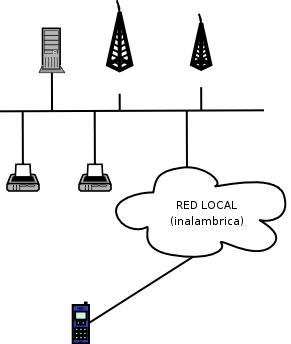
\includegraphics[scale=0.5]{DiagramaRed.png} } 
     	\end{center}
    	\caption{Diagrama de red}
	\label{fig:diaRed}
\end{figure*}

La distribuci'on de los puntos de acceso se debe realizar ubic'andolos en las esquinas de unos cuadradros imaginarios. El n'umero de puntos y dispostivos  perif'ericos depende del tamaño de la planta. Un ejemplo de planta ser'ia el de la figura \ref{fig:diaPlantaRed}.
\begin{figure*}[h!]
	\begin{center}
        		\framebox{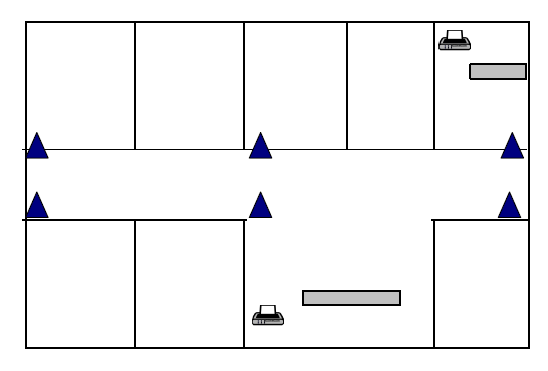
\includegraphics[scale=0.5]{plantaRed.png} } 
     	\end{center}
    	\caption{Mapa de una planta}
	\label{fig:diaPlantaRed}
\end{figure*}